\documentclass[]{article}
\usepackage{lmodern}
\usepackage{amssymb,amsmath}
\usepackage{ifxetex,ifluatex}
\usepackage{fixltx2e} % provides \textsubscript
\ifnum 0\ifxetex 1\fi\ifluatex 1\fi=0 % if pdftex
  \usepackage[T1]{fontenc}
  \usepackage[utf8]{inputenc}
\else % if luatex or xelatex
  \ifxetex
    \usepackage{mathspec}
  \else
    \usepackage{fontspec}
  \fi
  \defaultfontfeatures{Ligatures=TeX,Scale=MatchLowercase}
\fi
% use upquote if available, for straight quotes in verbatim environments
\IfFileExists{upquote.sty}{\usepackage{upquote}}{}
% use microtype if available
\IfFileExists{microtype.sty}{%
\usepackage{microtype}
\UseMicrotypeSet[protrusion]{basicmath} % disable protrusion for tt fonts
}{}
\usepackage[margin=1in]{geometry}
\usepackage{hyperref}
\hypersetup{unicode=true,
            pdftitle={Yinan\_Kang\_PS1},
            pdfauthor={Yinan Kang (yik398@g.harvard.edu)},
            pdfborder={0 0 0},
            breaklinks=true}
\urlstyle{same}  % don't use monospace font for urls
\usepackage{color}
\usepackage{fancyvrb}
\newcommand{\VerbBar}{|}
\newcommand{\VERB}{\Verb[commandchars=\\\{\}]}
\DefineVerbatimEnvironment{Highlighting}{Verbatim}{commandchars=\\\{\}}
% Add ',fontsize=\small' for more characters per line
\usepackage{framed}
\definecolor{shadecolor}{RGB}{248,248,248}
\newenvironment{Shaded}{\begin{snugshade}}{\end{snugshade}}
\newcommand{\AlertTok}[1]{\textcolor[rgb]{0.94,0.16,0.16}{#1}}
\newcommand{\AnnotationTok}[1]{\textcolor[rgb]{0.56,0.35,0.01}{\textbf{\textit{#1}}}}
\newcommand{\AttributeTok}[1]{\textcolor[rgb]{0.77,0.63,0.00}{#1}}
\newcommand{\BaseNTok}[1]{\textcolor[rgb]{0.00,0.00,0.81}{#1}}
\newcommand{\BuiltInTok}[1]{#1}
\newcommand{\CharTok}[1]{\textcolor[rgb]{0.31,0.60,0.02}{#1}}
\newcommand{\CommentTok}[1]{\textcolor[rgb]{0.56,0.35,0.01}{\textit{#1}}}
\newcommand{\CommentVarTok}[1]{\textcolor[rgb]{0.56,0.35,0.01}{\textbf{\textit{#1}}}}
\newcommand{\ConstantTok}[1]{\textcolor[rgb]{0.00,0.00,0.00}{#1}}
\newcommand{\ControlFlowTok}[1]{\textcolor[rgb]{0.13,0.29,0.53}{\textbf{#1}}}
\newcommand{\DataTypeTok}[1]{\textcolor[rgb]{0.13,0.29,0.53}{#1}}
\newcommand{\DecValTok}[1]{\textcolor[rgb]{0.00,0.00,0.81}{#1}}
\newcommand{\DocumentationTok}[1]{\textcolor[rgb]{0.56,0.35,0.01}{\textbf{\textit{#1}}}}
\newcommand{\ErrorTok}[1]{\textcolor[rgb]{0.64,0.00,0.00}{\textbf{#1}}}
\newcommand{\ExtensionTok}[1]{#1}
\newcommand{\FloatTok}[1]{\textcolor[rgb]{0.00,0.00,0.81}{#1}}
\newcommand{\FunctionTok}[1]{\textcolor[rgb]{0.00,0.00,0.00}{#1}}
\newcommand{\ImportTok}[1]{#1}
\newcommand{\InformationTok}[1]{\textcolor[rgb]{0.56,0.35,0.01}{\textbf{\textit{#1}}}}
\newcommand{\KeywordTok}[1]{\textcolor[rgb]{0.13,0.29,0.53}{\textbf{#1}}}
\newcommand{\NormalTok}[1]{#1}
\newcommand{\OperatorTok}[1]{\textcolor[rgb]{0.81,0.36,0.00}{\textbf{#1}}}
\newcommand{\OtherTok}[1]{\textcolor[rgb]{0.56,0.35,0.01}{#1}}
\newcommand{\PreprocessorTok}[1]{\textcolor[rgb]{0.56,0.35,0.01}{\textit{#1}}}
\newcommand{\RegionMarkerTok}[1]{#1}
\newcommand{\SpecialCharTok}[1]{\textcolor[rgb]{0.00,0.00,0.00}{#1}}
\newcommand{\SpecialStringTok}[1]{\textcolor[rgb]{0.31,0.60,0.02}{#1}}
\newcommand{\StringTok}[1]{\textcolor[rgb]{0.31,0.60,0.02}{#1}}
\newcommand{\VariableTok}[1]{\textcolor[rgb]{0.00,0.00,0.00}{#1}}
\newcommand{\VerbatimStringTok}[1]{\textcolor[rgb]{0.31,0.60,0.02}{#1}}
\newcommand{\WarningTok}[1]{\textcolor[rgb]{0.56,0.35,0.01}{\textbf{\textit{#1}}}}
\usepackage{graphicx,grffile}
\makeatletter
\def\maxwidth{\ifdim\Gin@nat@width>\linewidth\linewidth\else\Gin@nat@width\fi}
\def\maxheight{\ifdim\Gin@nat@height>\textheight\textheight\else\Gin@nat@height\fi}
\makeatother
% Scale images if necessary, so that they will not overflow the page
% margins by default, and it is still possible to overwrite the defaults
% using explicit options in \includegraphics[width, height, ...]{}
\setkeys{Gin}{width=\maxwidth,height=\maxheight,keepaspectratio}
\IfFileExists{parskip.sty}{%
\usepackage{parskip}
}{% else
\setlength{\parindent}{0pt}
\setlength{\parskip}{6pt plus 2pt minus 1pt}
}
\setlength{\emergencystretch}{3em}  % prevent overfull lines
\providecommand{\tightlist}{%
  \setlength{\itemsep}{0pt}\setlength{\parskip}{0pt}}
\setcounter{secnumdepth}{0}
% Redefines (sub)paragraphs to behave more like sections
\ifx\paragraph\undefined\else
\let\oldparagraph\paragraph
\renewcommand{\paragraph}[1]{\oldparagraph{#1}\mbox{}}
\fi
\ifx\subparagraph\undefined\else
\let\oldsubparagraph\subparagraph
\renewcommand{\subparagraph}[1]{\oldsubparagraph{#1}\mbox{}}
\fi

%%% Use protect on footnotes to avoid problems with footnotes in titles
\let\rmarkdownfootnote\footnote%
\def\footnote{\protect\rmarkdownfootnote}

%%% Change title format to be more compact
\usepackage{titling}

% Create subtitle command for use in maketitle
\providecommand{\subtitle}[1]{
  \posttitle{
    \begin{center}\large#1\end{center}
    }
}

\setlength{\droptitle}{-2em}

  \title{Yinan\_Kang\_PS1}
    \pretitle{\vspace{\droptitle}\centering\huge}
  \posttitle{\par}
    \author{Yinan Kang
(\href{mailto:yik398@g.harvard.edu}{\nolinkurl{yik398@g.harvard.edu}})}
    \preauthor{\centering\large\emph}
  \postauthor{\par}
    \date{}
    \predate{}\postdate{}
  

\begin{document}
\maketitle

\hypertarget{data}{%
\subsubsection{Data}\label{data}}

We will be using the
\href{https://www1.nyc.gov/site/nypd/stats/reports-analysis/stopfrisk.page}{Stop,
Question and Frisk Data from the NYPD} which contains information about
over 100,000 police citizen interactions between 2003-2016.

\begin{Shaded}
\begin{Highlighting}[]
\CommentTok{# Let's first load the R packages and the data}
\KeywordTok{library}\NormalTok{(bitops)}
\KeywordTok{library}\NormalTok{(foreign)}
\KeywordTok{library}\NormalTok{(RCurl)}


\NormalTok{stopandfrisk2016<-}
\StringTok{  }\KeywordTok{read.csv}\NormalTok{(}
    \DataTypeTok{text=}\KeywordTok{getURL}\NormalTok{(}\StringTok{"https://raw.githubusercontent.com/ljanastas/WWS586A-Machine-Learning-Policy-Analysis/master/Data/stop-and-frisk2016.csv"}\NormalTok{),  }
           \DataTypeTok{header=}\NormalTok{T)}
\end{Highlighting}
\end{Shaded}

\hypertarget{background}{%
\subsubsection{Background}\label{background}}

Bill DeBlasio has come to you because he is interested in conducting an
audit of some of the NYPD's policies for frisking individuals suspected
of criminar activity. He is particularly concerned that those indivduals
that are frisked happen to be overwhelmingly African-American.

\hypertarget{summary-statistics-30-points}{%
\subsubsection{1: Summary statistics (30
Points)}\label{summary-statistics-30-points}}

As a first cut, DeBlasio would like to see summary statistics (\(%
\) of people frisked and \(%
\) of people not frisked) within each racial category.

In other words, of the people that are frisked, what percent are Black,
White, Hispanic etc. Of the people that are not frisked, what percent
are Black, White, Hispanic etc..

\begin{Shaded}
\begin{Highlighting}[]
\KeywordTok{attach}\NormalTok{(stopandfrisk2016)}
\KeywordTok{library}\NormalTok{(dplyr)}
\end{Highlighting}
\end{Shaded}

\begin{verbatim}
## 
## Attaching package: 'dplyr'
\end{verbatim}

\begin{verbatim}
## The following objects are masked from 'package:stats':
## 
##     filter, lag
\end{verbatim}

\begin{verbatim}
## The following objects are masked from 'package:base':
## 
##     intersect, setdiff, setequal, union
\end{verbatim}

\begin{Shaded}
\begin{Highlighting}[]
\CommentTok{# Check what Races were recorded, and if any NA's exist }
\KeywordTok{unique}\NormalTok{(race)}
\end{Highlighting}
\end{Shaded}

\begin{verbatim}
## [1] B W P A Q U Z I  
## Levels:   A B I P Q U W Z
\end{verbatim}

\begin{Shaded}
\begin{Highlighting}[]
\KeywordTok{any}\NormalTok{(}\KeywordTok{is.na}\NormalTok{(race))}
\end{Highlighting}
\end{Shaded}

\begin{verbatim}
## [1] FALSE
\end{verbatim}

\begin{Shaded}
\begin{Highlighting}[]
\CommentTok{# Subset those who were frisked and not frisked}
\NormalTok{f <-}\StringTok{ }\NormalTok{stopandfrisk2016[frisked}\OperatorTok{==}\StringTok{"Y"}\NormalTok{,]}
\NormalTok{n <-}\StringTok{ }\NormalTok{stopandfrisk2016[frisked}\OperatorTok{==}\StringTok{"N"}\NormalTok{,]}

\NormalTok{f.a <-}\StringTok{ }\KeywordTok{nrow}\NormalTok{(f[f}\OperatorTok{$}\NormalTok{race}\OperatorTok{==}\StringTok{"A"}\NormalTok{,]) }\OperatorTok{/}\StringTok{ }\KeywordTok{nrow}\NormalTok{(f) }\OperatorTok{*}\StringTok{ }\DecValTok{100} 
\NormalTok{f.b <-}\StringTok{ }\KeywordTok{nrow}\NormalTok{(f[f}\OperatorTok{$}\NormalTok{race}\OperatorTok{==}\StringTok{"B"}\NormalTok{,]) }\OperatorTok{/}\StringTok{ }\KeywordTok{nrow}\NormalTok{(f) }\OperatorTok{*}\StringTok{ }\DecValTok{100} 
\NormalTok{f.i <-}\StringTok{ }\KeywordTok{nrow}\NormalTok{(f[f}\OperatorTok{$}\NormalTok{race}\OperatorTok{==}\StringTok{"I"}\NormalTok{,]) }\OperatorTok{/}\StringTok{ }\KeywordTok{nrow}\NormalTok{(f) }\OperatorTok{*}\StringTok{ }\DecValTok{100} 
\NormalTok{f.p <-}\StringTok{ }\KeywordTok{nrow}\NormalTok{(f[f}\OperatorTok{$}\NormalTok{race}\OperatorTok{==}\StringTok{"P"}\NormalTok{,]) }\OperatorTok{/}\StringTok{ }\KeywordTok{nrow}\NormalTok{(f) }\OperatorTok{*}\StringTok{ }\DecValTok{100} 
\NormalTok{f.q <-}\StringTok{ }\KeywordTok{nrow}\NormalTok{(f[f}\OperatorTok{$}\NormalTok{race}\OperatorTok{==}\StringTok{"Q"}\NormalTok{,]) }\OperatorTok{/}\StringTok{ }\KeywordTok{nrow}\NormalTok{(f) }\OperatorTok{*}\StringTok{ }\DecValTok{100} 
\NormalTok{f.u <-}\StringTok{ }\KeywordTok{nrow}\NormalTok{(f[f}\OperatorTok{$}\NormalTok{race}\OperatorTok{==}\StringTok{"U"}\NormalTok{,]) }\OperatorTok{/}\StringTok{ }\KeywordTok{nrow}\NormalTok{(f) }\OperatorTok{*}\StringTok{ }\DecValTok{100} 
\NormalTok{f.w <-}\StringTok{ }\KeywordTok{nrow}\NormalTok{(f[f}\OperatorTok{$}\NormalTok{race}\OperatorTok{==}\StringTok{"W"}\NormalTok{,]) }\OperatorTok{/}\StringTok{ }\KeywordTok{nrow}\NormalTok{(f) }\OperatorTok{*}\StringTok{ }\DecValTok{100} 
\NormalTok{f.z <-}\StringTok{ }\KeywordTok{nrow}\NormalTok{(f[f}\OperatorTok{$}\NormalTok{race}\OperatorTok{==}\StringTok{"Z"}\NormalTok{,]) }\OperatorTok{/}\StringTok{ }\KeywordTok{nrow}\NormalTok{(f) }\OperatorTok{*}\StringTok{ }\DecValTok{100} 

\NormalTok{n.a <-}\StringTok{ }\KeywordTok{nrow}\NormalTok{(n[n}\OperatorTok{$}\NormalTok{race}\OperatorTok{==}\StringTok{"A"}\NormalTok{,]) }\OperatorTok{/}\StringTok{ }\KeywordTok{nrow}\NormalTok{(n) }\OperatorTok{*}\StringTok{ }\DecValTok{100} 
\NormalTok{n.b <-}\StringTok{ }\KeywordTok{nrow}\NormalTok{(n[n}\OperatorTok{$}\NormalTok{race}\OperatorTok{==}\StringTok{"B"}\NormalTok{,]) }\OperatorTok{/}\StringTok{ }\KeywordTok{nrow}\NormalTok{(n) }\OperatorTok{*}\StringTok{ }\DecValTok{100} 
\NormalTok{n.i <-}\StringTok{ }\KeywordTok{nrow}\NormalTok{(n[n}\OperatorTok{$}\NormalTok{race}\OperatorTok{==}\StringTok{"I"}\NormalTok{,]) }\OperatorTok{/}\StringTok{ }\KeywordTok{nrow}\NormalTok{(n) }\OperatorTok{*}\StringTok{ }\DecValTok{100} 
\NormalTok{n.p <-}\StringTok{ }\KeywordTok{nrow}\NormalTok{(n[n}\OperatorTok{$}\NormalTok{race}\OperatorTok{==}\StringTok{"P"}\NormalTok{,]) }\OperatorTok{/}\StringTok{ }\KeywordTok{nrow}\NormalTok{(n) }\OperatorTok{*}\StringTok{ }\DecValTok{100} 
\NormalTok{n.q <-}\StringTok{ }\KeywordTok{nrow}\NormalTok{(n[n}\OperatorTok{$}\NormalTok{race}\OperatorTok{==}\StringTok{"Q"}\NormalTok{,]) }\OperatorTok{/}\StringTok{ }\KeywordTok{nrow}\NormalTok{(n) }\OperatorTok{*}\StringTok{ }\DecValTok{100} 
\NormalTok{n.u <-}\StringTok{ }\KeywordTok{nrow}\NormalTok{(n[n}\OperatorTok{$}\NormalTok{race}\OperatorTok{==}\StringTok{"U"}\NormalTok{,]) }\OperatorTok{/}\StringTok{ }\KeywordTok{nrow}\NormalTok{(n) }\OperatorTok{*}\StringTok{ }\DecValTok{100} 
\NormalTok{n.w <-}\StringTok{ }\KeywordTok{nrow}\NormalTok{(n[n}\OperatorTok{$}\NormalTok{race}\OperatorTok{==}\StringTok{"W"}\NormalTok{,]) }\OperatorTok{/}\StringTok{ }\KeywordTok{nrow}\NormalTok{(n) }\OperatorTok{*}\StringTok{ }\DecValTok{100} 
\NormalTok{n.z <-}\StringTok{ }\KeywordTok{nrow}\NormalTok{(n[n}\OperatorTok{$}\NormalTok{race}\OperatorTok{==}\StringTok{"Z"}\NormalTok{,]) }\OperatorTok{/}\StringTok{ }\KeywordTok{nrow}\NormalTok{(n) }\OperatorTok{*}\StringTok{ }\DecValTok{100} 
\end{Highlighting}
\end{Shaded}

\textbf{Summary of Results}:

Of those Frisked:\\
5.4792795\% were Race A\\
54.6164504\% were Race B\\
0.2645169\% were Race I\\
7.3560902\% were Race P\\
22.3201915\% were Race Q\\
0.6046102\% were Race U\\
8.3007936\% were Race W\\
1.0580678\% were Race Z

Of those Not Frisked:\\
6.7637178\% were Race A\\
48.4210526\% were Race B\\
0.3807391\% were Race I\\
6.4725644\% were Race P\\
21.9708847\% were Race Q\\
1.0526316\% were Race U\\
13.6842105\% were Race W\\
1.2541993\% were Race Z

\hypertarget{visualization-30-points}{%
\subsubsection{2: Visualization (30
Points)}\label{visualization-30-points}}

In addition to the summary statistics, the mayor would like you to
produce two plots: a pie chart and a bar plot containing the percent of
people within each racial group that were frisked.

Both the pie chart and the bar plot should have the title ``Percent of
Racial Group Frisked''.

Also, please save both plots as .png files. No need to submit the
images, just make sure that the code is included below.

\begin{Shaded}
\begin{Highlighting}[]
\CommentTok{# Creating inputs for graphs}
\NormalTok{slices <-}\StringTok{ }\KeywordTok{c}\NormalTok{(f.a,f.b,f.i,f.p,f.q,f.u,f.w,f.z)}
\NormalTok{lbls <-}\StringTok{ }\KeywordTok{c}\NormalTok{(}\StringTok{"A"}\NormalTok{,}\StringTok{"B"}\NormalTok{,}\StringTok{"I"}\NormalTok{,}\StringTok{"P"}\NormalTok{,}\StringTok{"Q"}\NormalTok{,}\StringTok{"U"}\NormalTok{,}\StringTok{"W"}\NormalTok{,}\StringTok{"Z"}\NormalTok{)}

\CommentTok{# Setting up png export, and generating graphs}
\NormalTok{pie <-}\StringTok{ }\KeywordTok{pie}\NormalTok{(slices,lbls, }\DataTypeTok{main =} \StringTok{"Percent of Racial Group Frisked"}\NormalTok{)}
\end{Highlighting}
\end{Shaded}

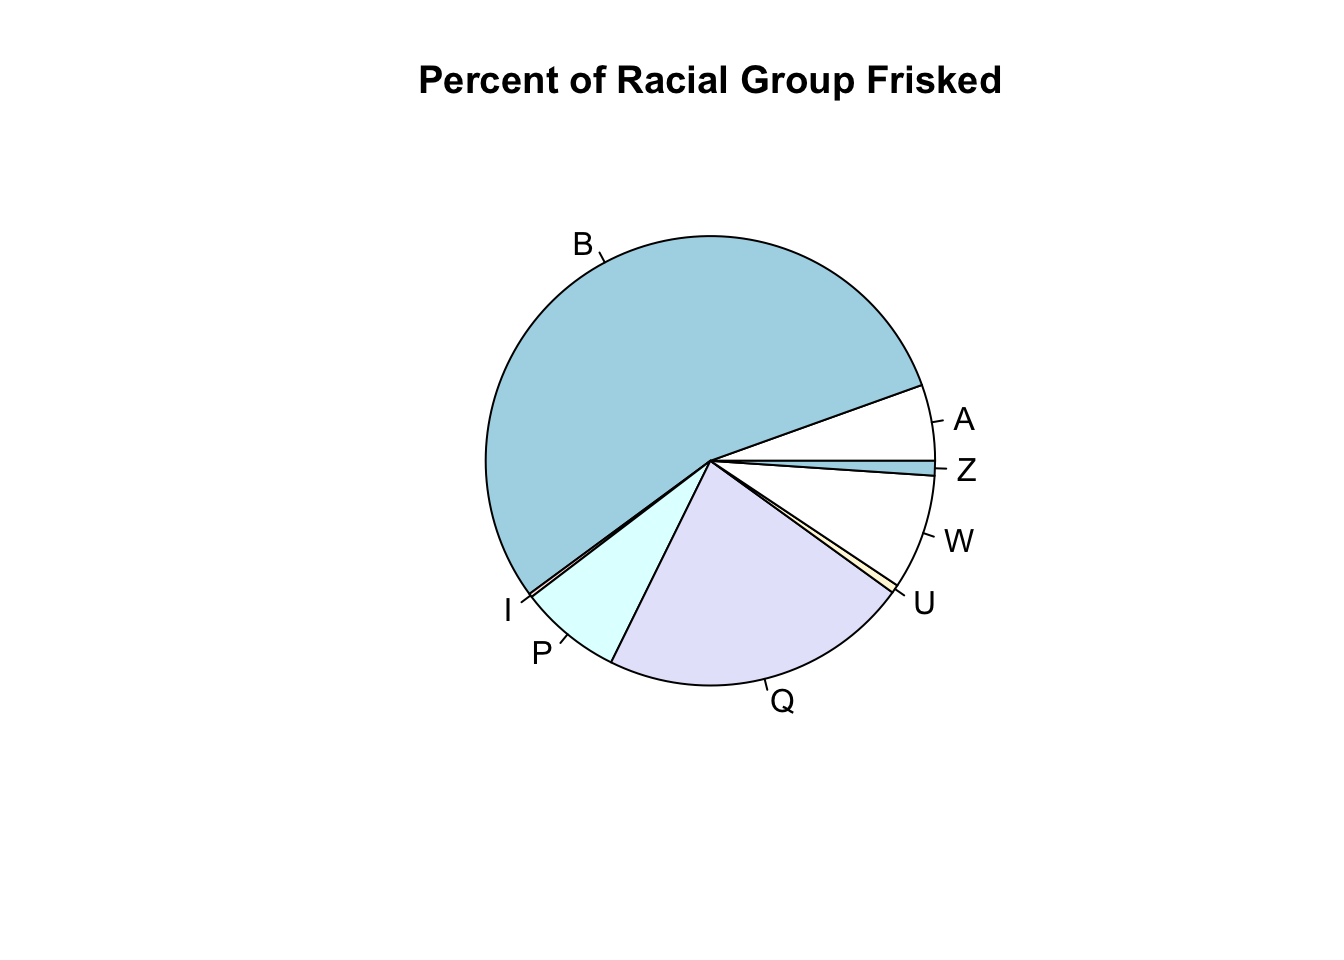
\includegraphics{yinan_kang_ps1_files/figure-latex/unnamed-chunk-3-1.pdf}

\begin{Shaded}
\begin{Highlighting}[]
\NormalTok{bar <-}\StringTok{ }\KeywordTok{barplot}\NormalTok{(slices, }\DataTypeTok{names.arg =}\NormalTok{ lbls, }\DataTypeTok{main =} \StringTok{"Percent of Racial Group Frisked"}\NormalTok{)}
\end{Highlighting}
\end{Shaded}

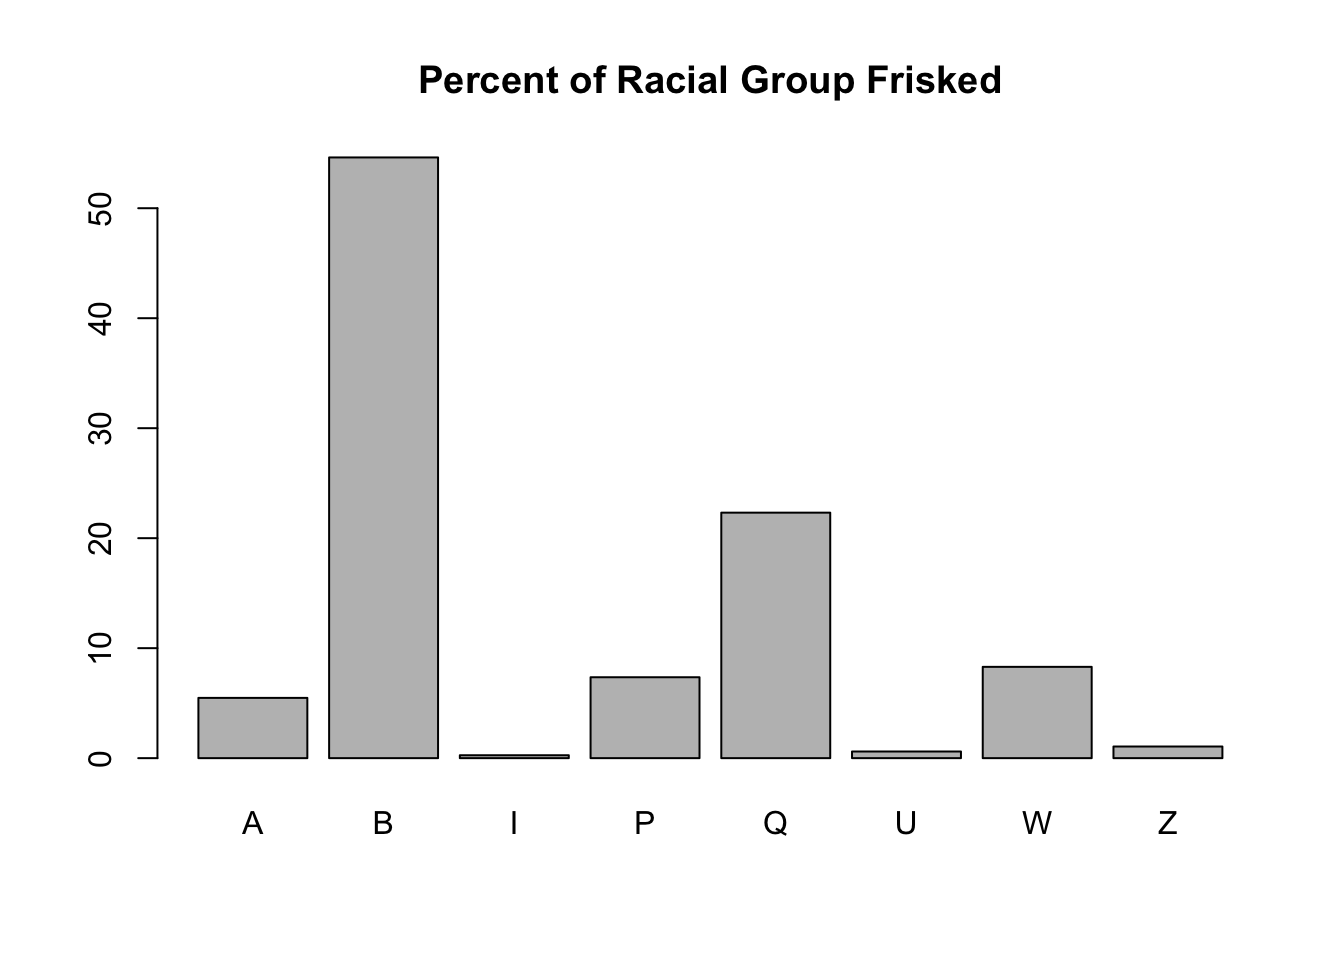
\includegraphics{yinan_kang_ps1_files/figure-latex/unnamed-chunk-3-2.pdf}

\begin{Shaded}
\begin{Highlighting}[]
\KeywordTok{png}\NormalTok{(}\StringTok{"pie.png"}\NormalTok{)}
\KeywordTok{pie}\NormalTok{(slices,lbls, }\DataTypeTok{main =} \StringTok{"Percent of Racial Group Frisked"}\NormalTok{)}
\KeywordTok{dev.off}\NormalTok{() }
\end{Highlighting}
\end{Shaded}

\begin{verbatim}
## pdf 
##   2
\end{verbatim}

\begin{Shaded}
\begin{Highlighting}[]
\KeywordTok{png}\NormalTok{(}\StringTok{"bar.png"}\NormalTok{)}
\KeywordTok{barplot}\NormalTok{(slices, }\DataTypeTok{names.arg =}\NormalTok{ lbls, }\DataTypeTok{main =} \StringTok{"Percent of Racial Group Frisked"}\NormalTok{)}
\KeywordTok{dev.off}\NormalTok{() }
\end{Highlighting}
\end{Shaded}

\begin{verbatim}
## pdf 
##   2
\end{verbatim}

\hypertarget{writing-functions-40-points}{%
\subsubsection{3: Writing functions (40
Points)}\label{writing-functions-40-points}}

Many of the variables in the stop and frisk data are coded as ``Y'' for
``Yes'' and ``N'' for no. You want to have an easy means of recoding
every variable in the stop and frisk data set using a function that you
define.

\hypertarget{a-20-points}{%
\paragraph{(a) (20 Points)}\label{a-20-points}}

In order to save some time from having to recode every single variable
that contains a ``Y'' or a ``N'', write a function that transforms:

\begin{itemize}
\tightlist
\item
  ``Y'' codings to ``1''
\item
  ``N'' codings to ``0''
\item
  " " codings to ``NA''
\end{itemize}

for a single variable and returns the recoded variable. Call this
function ``yesno''

\begin{Shaded}
\begin{Highlighting}[]
\CommentTok{# YOUR CODE HERE }
\CommentTok{# Added a 3rd function input, that'll be used for indexing purposes}
\NormalTok{yesno<-}\ControlFlowTok{function}\NormalTok{(oldvariable,newvariable,col)\{}
   \ControlFlowTok{if}\NormalTok{ (}\KeywordTok{any}\NormalTok{(oldvariable}\OperatorTok{==}\StringTok{"Y"}\NormalTok{) }\OperatorTok{==}\StringTok{ }\OtherTok{TRUE}\NormalTok{) \{}
      \ControlFlowTok{for}\NormalTok{ (i }\ControlFlowTok{in}\NormalTok{ (}\DecValTok{1}\OperatorTok{:}\KeywordTok{length}\NormalTok{(oldvariable)))\{}
        
        \ControlFlowTok{if}\NormalTok{ (oldvariable[i] }\OperatorTok{==}\StringTok{ "Y"}\NormalTok{)\{}
\NormalTok{        newvariable[i,col}\OperatorTok{+}\DecValTok{1}\NormalTok{] =}\StringTok{ "1"}
\NormalTok{        \}}
        \ControlFlowTok{if}\NormalTok{ (oldvariable[i] }\OperatorTok{==}\StringTok{ "N"}\NormalTok{)\{}
\NormalTok{        newvariable[i,col}\OperatorTok{+}\DecValTok{1}\NormalTok{] =}\StringTok{ "0"}
\NormalTok{        \}}
        \ControlFlowTok{if}\NormalTok{ (oldvariable[i] }\OperatorTok{==}\StringTok{ " "}\NormalTok{)\{}
\NormalTok{        newvariable[i,col}\OperatorTok{+}\DecValTok{1}\NormalTok{] =}\StringTok{ "NA"} 
\NormalTok{        \}}
        \ControlFlowTok{else}\NormalTok{ \{(}\ControlFlowTok{next}\NormalTok{())\}}

\NormalTok{      \}}
\NormalTok{    \}}
  \CommentTok{# else\{print('nope')\} was using this to troubleshoot earlier}
  \KeywordTok{return}\NormalTok{(newvariable)}
\NormalTok{\}}
\end{Highlighting}
\end{Shaded}

\hypertarget{b-20-points}{%
\paragraph{(b) (20 Points)}\label{b-20-points}}

Using the function that you defined in part (a), write a loop that
transforms every single variable in the ``stopandfrisk2016'' data frame
containing a ``Y'' or ``N'' coding into ``1'', ``0'' or ``NA'' codings
as specified above.

Save these newly coded variables in a data frame called ``recoded'' and
use the ``head()'' function to print out the first few observations of
the new dataframe that you created.

\begin{Shaded}
\begin{Highlighting}[]
\CommentTok{# Initiate empty 'recoded' data frame }
\NormalTok{recoded <-}\StringTok{ }\KeywordTok{data.frame}\NormalTok{()}
\CommentTok{# nope=0 ... was using this for troubleshooting }

\CommentTok{# Creating loop that will send in columsn of 'stopandfrisk2016' as inputs, 'recoded' results dataframe as output, and also take in current iteration of}
\CommentTok{# number of columns in 'recoded' for indexing purposes }
\ControlFlowTok{for}\NormalTok{ (j }\ControlFlowTok{in} \DecValTok{1}\OperatorTok{:}\DecValTok{90}\NormalTok{)\{}
    \ControlFlowTok{if}\NormalTok{ (}\KeywordTok{is.factor}\NormalTok{(stopandfrisk2016[,j]) }\OperatorTok{==}\StringTok{ }\OtherTok{TRUE}\NormalTok{)\{}
\NormalTok{      recoded <-}\StringTok{ }\KeywordTok{yesno}\NormalTok{(stopandfrisk2016[,j],recoded,}\KeywordTok{ncol}\NormalTok{(recoded))}
\NormalTok{      col.name <-}\StringTok{ }\KeywordTok{colnames}\NormalTok{(stopandfrisk2016[j])}
      \KeywordTok{colnames}\NormalTok{(recoded)[}\KeywordTok{ncol}\NormalTok{(recoded)] <-}\StringTok{ }\NormalTok{col.name}
\NormalTok{    \}}
    \CommentTok{# else \{ ... ignore, used this part for troubleshoot}
     \CommentTok{# nope <- nope + 1}
     \CommentTok{# print(nope)\} }
\NormalTok{\}}

\CommentTok{# Manually skipped column #91, 'othrfeatr', which was particularly funky and gave the function issues. It wasn't a Y/N column anyway }

\ControlFlowTok{for}\NormalTok{ (j }\ControlFlowTok{in} \DecValTok{92}\OperatorTok{:}\DecValTok{112}\NormalTok{)\{}
    \ControlFlowTok{if}\NormalTok{ (}\KeywordTok{is.factor}\NormalTok{(stopandfrisk2016[,j]) }\OperatorTok{==}\StringTok{ }\OtherTok{TRUE}\NormalTok{)\{}
\NormalTok{      recoded <-}\StringTok{ }\KeywordTok{yesno}\NormalTok{(stopandfrisk2016[,j],recoded,}\KeywordTok{ncol}\NormalTok{(recoded))}
\NormalTok{      col.name <-}\StringTok{ }\KeywordTok{colnames}\NormalTok{(stopandfrisk2016[j])}
      \KeywordTok{colnames}\NormalTok{(recoded)[}\KeywordTok{ncol}\NormalTok{(recoded)] <-}\StringTok{ }\NormalTok{col.name}
\NormalTok{    \}}
    \CommentTok{#else \{}
     \CommentTok{# nope <- nope + 1}
     \CommentTok{# print(nope)\} ... was using this section to troubleshoot earlier}
\NormalTok{\}}

\CommentTok{# Verifying the 'recoded' dataframe conversion worked}
\KeywordTok{head}\NormalTok{(recoded,}\DecValTok{8}\NormalTok{)}
\end{Highlighting}
\end{Shaded}

\begin{verbatim}
##   explnstp othpers arstoffn sumoffen officrid frisked searched adtlrept
## 1        1       0        0        1        0       1        1        0
## 2        1       1        0        0        0       0        1        0
## 3        1       0        1        0        1       1        1        0
## 4        1       0        0        0        1       1        0        0
## 5        1       0        0        0        1       0        0        0
## 6        1       0        0        0        1       1        0        0
## 7        1       0        0        0        1       1        0        0
## 8        1       0        0        0        0       1        0        0
##   pistol riflshot asltweap machgun othrweap pf_hands pf_wall pf_grnd
## 1      0        0        0       0        0        0       0       0
## 2      0        0        0       0        0        1       1       0
## 3      0        0        0       0        0        0       0       0
## 4      0        0        0       0        0        1       0       0
## 5      0        0        0       0        0        0       0       0
## 6      0        0        0       0        0        0       0       0
## 7      0        0        0       0        0        0       0       0
## 8      0        0        0       0        0        0       0       0
##   pf_drwep pf_ptwep pf_baton pf_hcuff pf_pepsp pf_other radio ac_rept
## 1        0        0        0        1        0        0     0       0
## 2        0        0        0        0        0        0     1       0
## 3        0        0        0        0        0        0     1       1
## 4        0        1        0        1        0        0     0       0
## 5        0        0        0        0        0        0     0       0
## 6        0        0        0        0        0        0     0       0
## 7        1        0        0        1        0        0     1       1
## 8        0        0        0        0        0        0     1       1
##   ac_inves rf_vcrim rf_othsw ac_proxm rf_attir cs_objcs cs_descr cs_casng
## 1        0        0        0        0        0        0        0        1
## 2        0        0        0        0        0        0        0        0
## 3        0        0        1        0        0        0        1        0
## 4        0        1        0        1        0        0        1        0
## 5        0        0        0        0        0        0        0        0
## 6        1        0        1        0        0        0        0        0
## 7        1        1        1        1        0        0        1        0
## 8        1        1        0        1        0        0        1        1
##   cs_lkout rf_vcact cs_cloth cs_drgtr ac_evasv ac_assoc cs_furtv rf_rfcmp
## 1        0        0        0        0        0        1        1        0
## 2        0        0        0        1        1        0        1        0
## 3        0        0        0        0        0        0        0        0
## 4        0        0        0        0        0        0        1        1
## 5        0        0        0        0        0        0        0        0
## 6        0        0        0        0        1        0        0        0
## 7        0        0        0        0        0        0        0        0
## 8        1        0        0        0        1        0        0        1
##   ac_cgdir rf_verbl cs_vcrim cs_bulge cs_other ac_incid ac_time rf_knowl
## 1        1        0        0        0        0        1       1        0
## 2        0        0        0        0        1        1       1        0
## 3        0        0        0        0        0        0       0        0
## 4        1        0        0        0        0        0       0        0
## 5        0        0        0        0        1        0       0        0
## 6        0        0        0        0        1        1       0        0
## 7        0        0        0        0        0        0       0        0
## 8        1        0        1        0        0        1       1        0
##   ac_stsnd ac_other sb_hdobj sb_outln sb_admis sb_other rf_furt dettypCM
## 1        0        0        0        0        0        1       1        0
## 2        0        0        0        0        0        1       0        0
## 3        0        0        0        0        0        1       0        0
## 4        0        0        0        0        0        0       1        0
## 5        0        1        0        0        0        0       0        0
## 6        0        0        0        0        0        0       0        0
## 7        0        0        0        0        0        0       0        0
## 8        0        0        0        0        0        0       0        0
\end{verbatim}

\begin{Shaded}
\begin{Highlighting}[]
\KeywordTok{colnames}\NormalTok{(recoded)}
\end{Highlighting}
\end{Shaded}

\begin{verbatim}
##  [1] "explnstp" "othpers"  "arstoffn" "sumoffen" "officrid" "frisked" 
##  [7] "searched" "adtlrept" "pistol"   "riflshot" "asltweap" "machgun" 
## [13] "othrweap" "pf_hands" "pf_wall"  "pf_grnd"  "pf_drwep" "pf_ptwep"
## [19] "pf_baton" "pf_hcuff" "pf_pepsp" "pf_other" "radio"    "ac_rept" 
## [25] "ac_inves" "rf_vcrim" "rf_othsw" "ac_proxm" "rf_attir" "cs_objcs"
## [31] "cs_descr" "cs_casng" "cs_lkout" "rf_vcact" "cs_cloth" "cs_drgtr"
## [37] "ac_evasv" "ac_assoc" "cs_furtv" "rf_rfcmp" "ac_cgdir" "rf_verbl"
## [43] "cs_vcrim" "cs_bulge" "cs_other" "ac_incid" "ac_time"  "rf_knowl"
## [49] "ac_stsnd" "ac_other" "sb_hdobj" "sb_outln" "sb_admis" "sb_other"
## [55] "rf_furt"  "dettypCM"
\end{verbatim}

\hypertarget{logistic-regression-extra-credit-10-points}{%
\subsubsection{4: Logistic regression (Extra Credit, 10
Points)}\label{logistic-regression-extra-credit-10-points}}

Estimate a logistic regression model using the ``frisked'' variable as
your dependent variable and with 5 independent variables of your
choosing. Calculate odds ratios for each of the independent variables
that you included in the model and print out the odds ratios.

Interpret the odds ratios for one your independent variables.

\begin{Shaded}
\begin{Highlighting}[]
\CommentTok{# Building a model and looking at summary}

\NormalTok{model <-}\StringTok{ }\KeywordTok{glm}\NormalTok{(frisked }\OperatorTok{~}\StringTok{ }\NormalTok{timestop }\OperatorTok{+}\StringTok{ }\NormalTok{pistol }\OperatorTok{+}\StringTok{ }\NormalTok{race }\OperatorTok{+}\StringTok{ }\NormalTok{sex }\OperatorTok{+}\StringTok{ }\NormalTok{build, }\DataTypeTok{data =}\NormalTok{ stopandfrisk2016, }\DataTypeTok{family =} \StringTok{"binomial"}\NormalTok{)}
\KeywordTok{summary}\NormalTok{(model)}
\end{Highlighting}
\end{Shaded}

\begin{verbatim}
## 
## Call:
## glm(formula = frisked ~ timestop + pistol + race + sex + build, 
##     family = "binomial", data = stopandfrisk2016)
## 
## Deviance Residuals: 
##     Min       1Q   Median       3Q      Max  
## -2.1596  -1.3679   0.8696   0.9066   1.7048  
## 
## Coefficients:
##               Estimate Std. Error z value Pr(>|z|)    
## (Intercept) -4.389e-01  1.229e-01  -3.572 0.000354 ***
## timestop     5.490e-05  2.477e-05   2.217 0.026646 *  
## pistolY      1.432e+00  2.460e-01   5.820 5.89e-09 ***
## raceB        3.316e-01  8.024e-02   4.133 3.59e-05 ***
## raceI       -1.620e-01  3.377e-01  -0.480 0.631478    
## raceP        3.352e-01  1.050e-01   3.194 0.001404 ** 
## raceQ        2.433e-01  8.570e-02   2.839 0.004527 ** 
## raceU       -3.266e-01  2.219e-01  -1.472 0.141035    
## raceW       -2.507e-01  9.464e-02  -2.649 0.008069 ** 
## raceZ        1.258e-01  2.036e-01   0.618 0.536584    
## sexM         1.047e+00  7.166e-02  14.606  < 2e-16 ***
## sexZ         7.848e-01  2.958e-01   2.653 0.007976 ** 
## buildM      -2.907e-01  6.971e-02  -4.169 3.05e-05 ***
## buildT      -2.577e-01  6.980e-02  -3.692 0.000222 ***
## buildU      -5.052e-01  1.913e-01  -2.641 0.008267 ** 
## buildZ      -6.132e-01  1.552e-01  -3.951 7.79e-05 ***
## ---
## Signif. codes:  0 '***' 0.001 '**' 0.01 '*' 0.05 '.' 0.1 ' ' 1
## 
## (Dispersion parameter for binomial family taken to be 1)
## 
##     Null deviance: 16209  on 12403  degrees of freedom
## Residual deviance: 15796  on 12388  degrees of freedom
##   (1 observation deleted due to missingness)
## AIC: 15828
## 
## Number of Fisher Scoring iterations: 4
\end{verbatim}

\begin{Shaded}
\begin{Highlighting}[]
\CommentTok{# Looking at odds ratio for 'raceB'}
\KeywordTok{exp}\NormalTok{(}\FloatTok{3.316e-01}\NormalTok{) }
\end{Highlighting}
\end{Shaded}

\begin{verbatim}
## [1] 1.393195
\end{verbatim}

\textbf{Odds Ratio}: Having race ``B'' increases odds of `frisked' by
1.39


\end{document}
